\documentclass[10pt,twocolumn]{article} 
\usepackage{simpleConference}
\usepackage{times}
\usepackage{graphicx}
\graphicspath{ {images/} }
\usepackage{amssymb}
\PassOptionsToPackage{hyphens}{url}\usepackage{hyperref}
\begin{document}

\title{Subterranean WiFi (SWIFT)}

\author{Amy Reed, Kristina Hager\\
Mobile Computing EE382V\\
University of Texas at Austin\\
\\
}

\maketitle
\thispagestyle{empty}

% \begin{abstract}
%    This is a simple sample of a document created using \LaTeX
%    (specifically pdflatex)
%    that includes a figure from the Vergil visual editor for Ptolemy II
%    that was created by printing to the Acrobat Distiller to get a PDF file.
%    It also illustrates a simple two-column conference paper style,
%    and use of bibtex to handle bibliographies.
% \end{abstract}

\section{Introduction}
Research takes scientists to places difficult to access to retrieve their study data. 
For this project, we will consider a common problem scientists face when doing research in caves involving sensors and associated data loggers. 
In-cave data loggers (sensors) collect data regarding CO2 levels, cave-drip water, temperature, humidity, and more. 
The most common method of retrieving this data from the data loggers in caves is via a human entering the cave, traveling to the collection site, and manually retrieving it. 
This method is very slow, inconvenient, and in some cases quite perilous. 
Furthermore, data loggers can and do malfunction.
A scientist will not know that her data logger has malfunctioned until she is able to visit the datalogger.
\begin{figure*}[t]
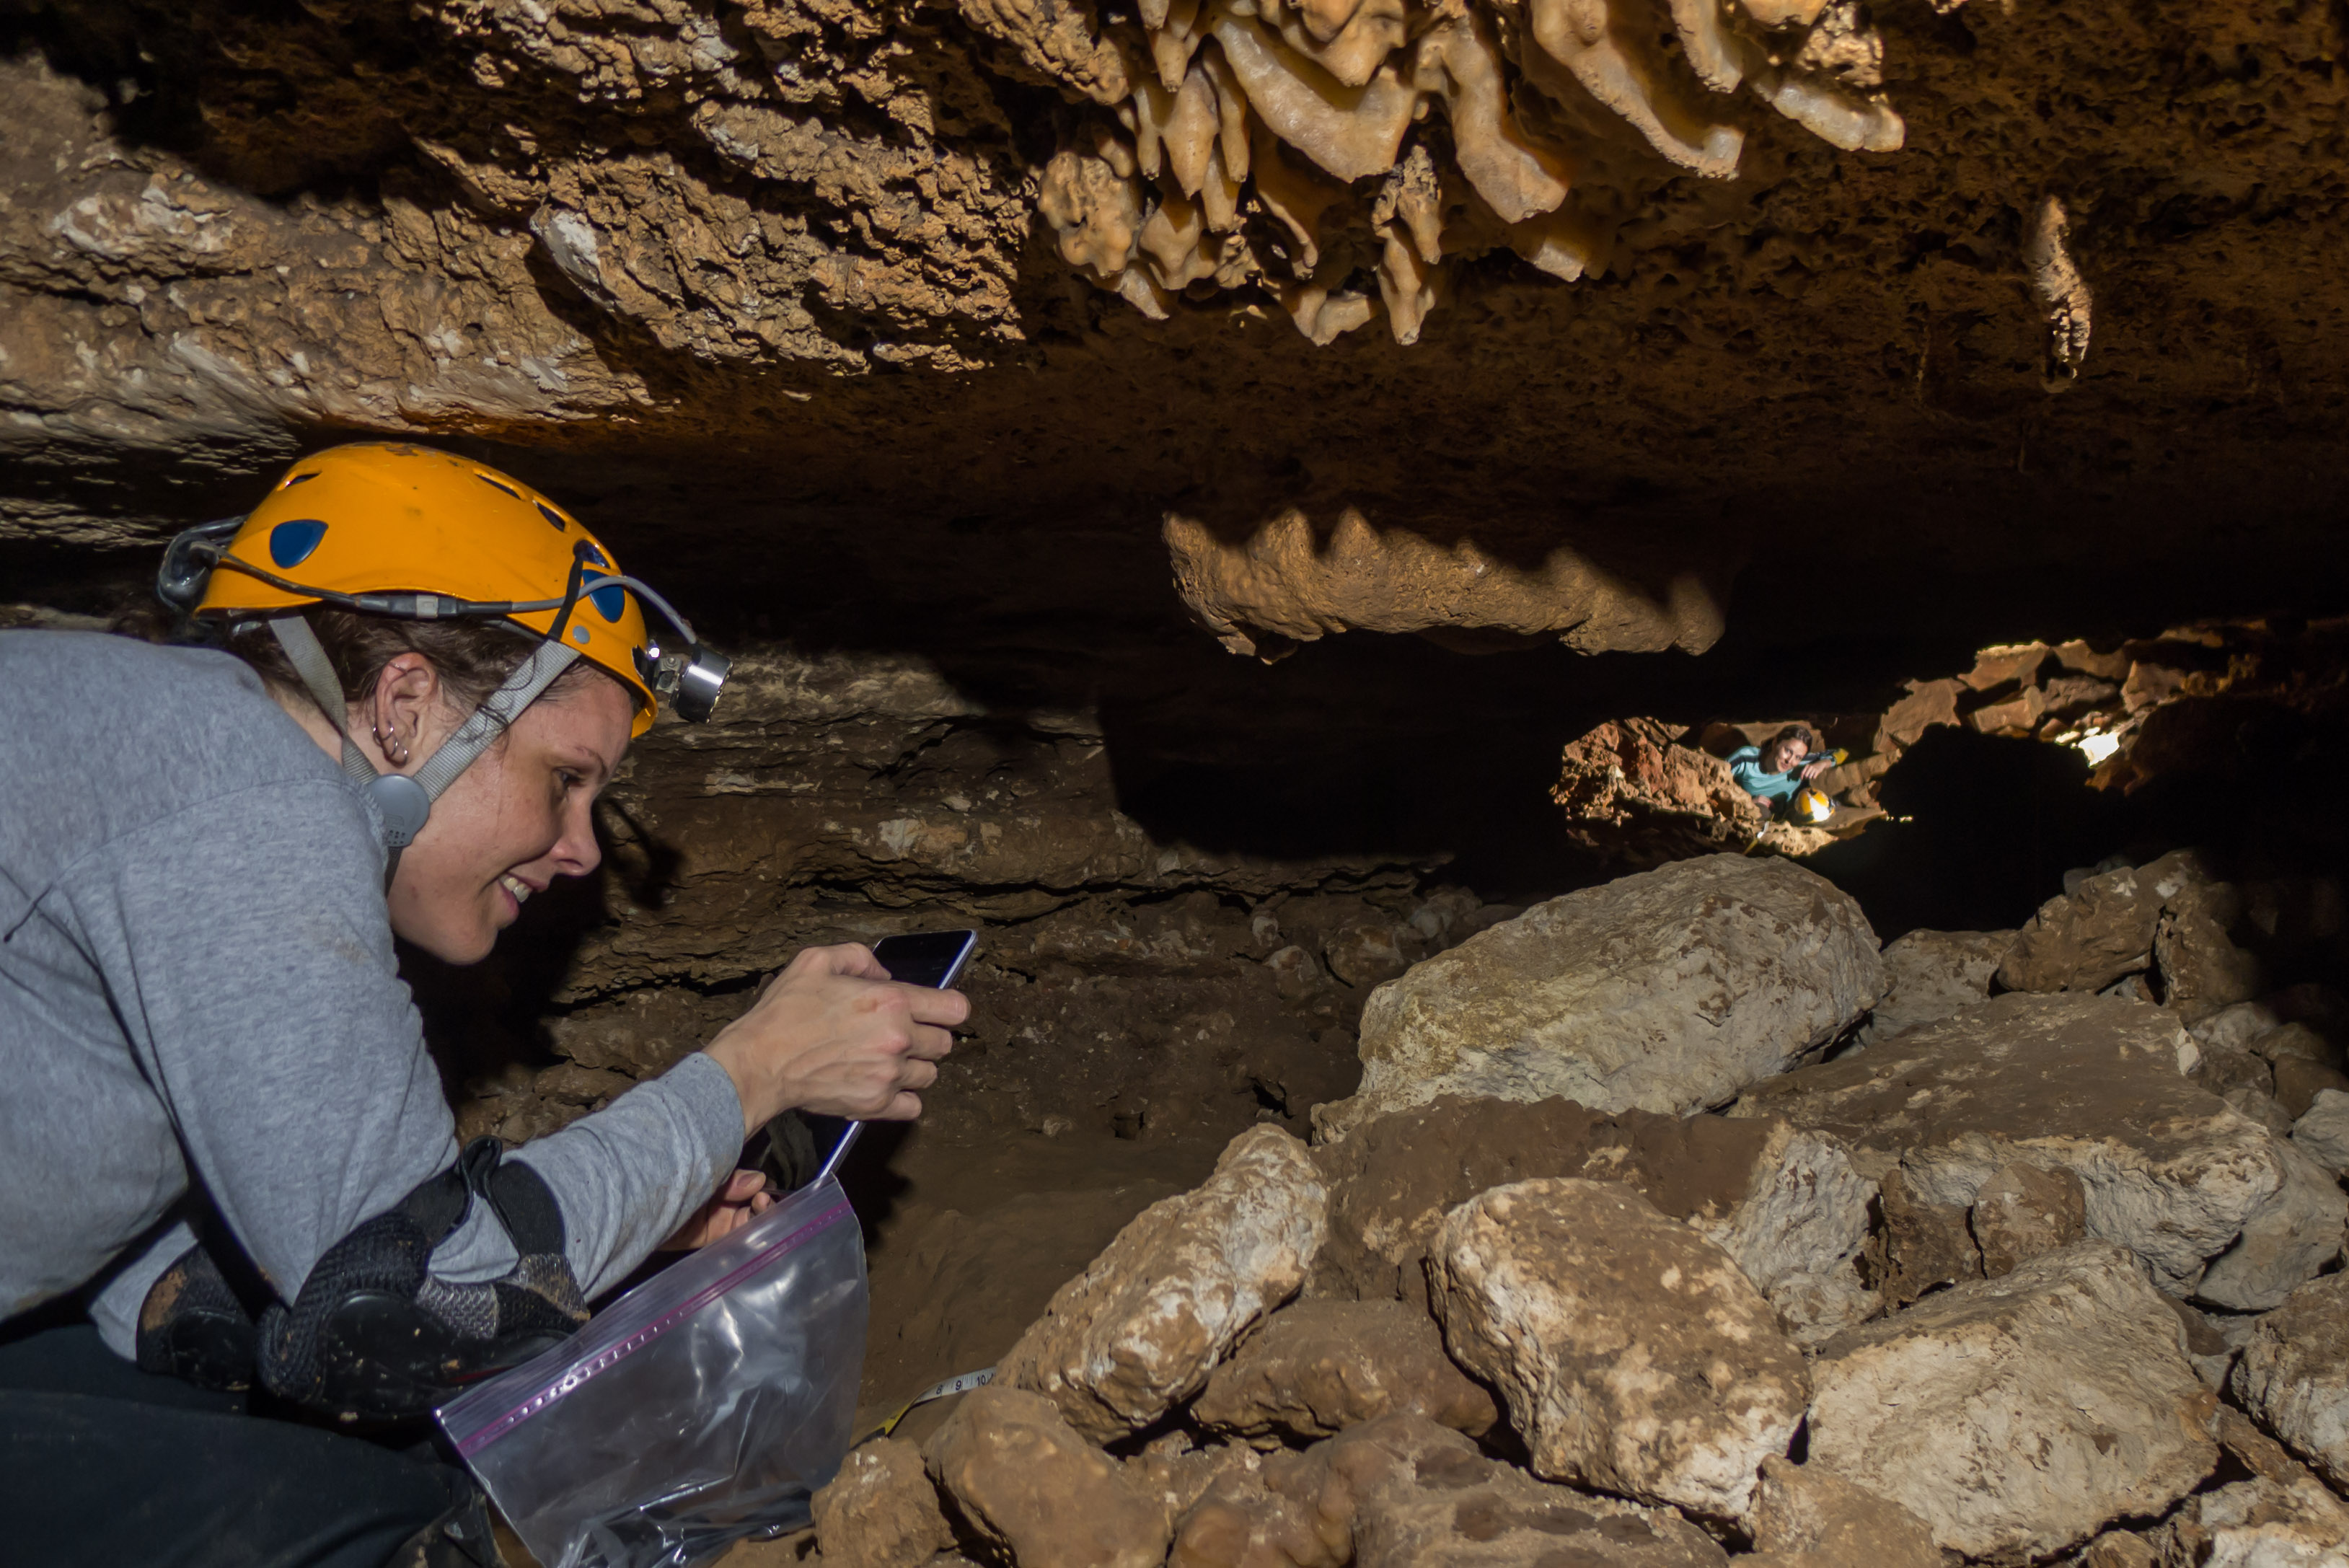
\includegraphics[width=\textwidth]{cavewifi2}
\end{figure*}
We propose a more automatic means of data retrieval from in-cave loggers. 
We propose to ferry data back to the surface using Wifi Direct enabled devices. 
This technology is now common in many mobile devices.
This would be a far more convenient, effective, and safe mechanism for data retrieval versus current techniques.  
The Wifi Direct standard provides infrastructure mechanisms for discovery, addressing, and security which could provide a simple and power effective means of setting up the network and transferring data. 

We will focus on two key questions in this paper regarding the potential of the Wifi Direct technology for this application.
First, we will investigate the range of the Wifi Direct technology in a cave environment.
WiFi Direct theoretically provides a range of up to 200m which is greater than that of Bluetooth technology. 
However, we would like to determine the potential range of Wifi Direct specifically in a cave environment which has different characteristics from a usual surface environment. 
Next, we will create a prototype application for ferrying data using Wifi Direct as provided by the Android platform. 
However, the still nascent implementation of the WiFi Direct APIs will pose some limitations for our use case.
The current implementation of Wifi Direct on Android devices does not allow a device to be simultaneously connected to two WifiDirect groups.
Since the data will need to travel from device to device, each device will need to participate in one or two groups. 
Since the connection to those groups cannot be simultaneous, our prototype application will manage the disconnect from one group and connect to the next group automatically.
In addition, the current wireless protected setup implementation requires the human user of the device to approve any new connections.
However, once a device has gained user permission once to a join a group, the Android platform "remembers" that permission and allows the device to automatically rejoin that group.
Since we want our devices to be able to operate autonomously underground, we will show how to accommodate the approval issue by pre-configuring the devices in their planned sequence.
 
For the first phase of this project, we created a prototype application for Android devices. 
We used this application to test the ability to make Wifi Direct connections within Whirlpool Cave, a popular cave in south Austin with a variety of passage characteristics. 
The ultimate goal of this initial application and the cave excursion is to determine if the range of Wifi Direct is sufficient to support passing messages out of the cave.
The results of this initial testing showed that WiFi Direct had significant range in areas where direct line of sight was achievable between devices.
We will discuss these experiments in a subsequent section of the paper.

For the second phase of the project, we will develop a second Android application to demonstrate how to pass a sample data file from device to device in a manner similar to how data would be ferried out of a cave.
While WiFi Direct can easily be used to transfer data files within a single WiFi Direct group, our application data transfer from peer to peer that extend beyond the range of what a single group can provide.
Ultimately the second application will determine if passing information from peer to peer to ferry the data from the cave is achievable. 
In addition to the key concern that the application could support multiple WiFi direct groups on the same device, we have concerns about timing of discovery and connectivity.
These must be implemented in such a way that a single wireless interface on the device can be shared.

We have not yet finished our research project. 
This paper serves to cover the progress that has been made thus far into answering the questions outlined in this introduction. 
% The remainder of this paper is structured as follows, section x�.

\section{Usage of sensors and data loggers in caves}

Many types of scientists such as geologists, hydrogeologists, climatologists and more conduct research in the interior of caves. 
These scientists are usually looking for information about the cave's microclimate and changes to the caves microclimate. 
For example, in \cite{wong2010}, the scientists are interested in monitoring changes in cave air CO$_2$ levels in response to brush clearing in areas above the cave. 

Caves present a wide variety of size and shape of passage and climate. 
Since power management is especially important for mobile devices WiFi direct includes power management mechanisms that can reduce power consumption for devices regardless of role.
For example, Son Doong Cave in Thailand has a large room that is over five kilometers long, 200 meters high and 150 meters wide \cite{sondoong}.

Most caves, however, are difficult and dangerous to some degree or another to access and data loggers are often placed deep in the cave.
Therefore, a researcher expends a great deal of time, logistics and even risk to her life when she needs to access her sensors and the data logger attached to the sensor.
Also, most cave climates have nearly 100\% humidity at all times and some caves flood or in general have conditions that make sensors and data loggers prone to failure.
When a sensor or data logger fails, the scientist loses a great deal of data which adds to the difficulty of cave research.
Therefore, cave researchers are interested in mechanisms that would make their data easier to access and available in a more timely manner.

\section{Related Work}SPWPS
Cave explorers and researchers need in cave communication systems in order to carry out complex group tasks such as expedition management, rescues, or photography projects.

Wired telephone technology is popular with expedition and rescue teams because they are simple and robust \cite{cavecomm}.
However, one major drawback of wire based systems is that the wire must be carefully laid along the cave passage. 
The wires themselves are heavy to carry and expensive.Also, if the wire is broken somewh
ere along the line, then the entire system will not work.
Therefore, the drawbacks of wired telephone technology are the cost and weight of the wire and fragility of the system.

The APRS Cave-Link system is capable of sending text based messages via VHF/UHF walkie talkies or relay boxes placed along a cave passage.
In their experiments in a large cave, the average hop length was an average of 390' and 440' for VHF and UHF respectively.
The advantages of this system over wired systems is that the radio units and relay boxes are approximately hand-sized and are relatively lightweight.
The authors were using the system to essentially send text messages and did not address the general data capacity of the system \cite{cavelink}.

In Postojna Cave in Slovenia, a research team created a system for delay tolerant automatic data transfer from environmental monitoring systems deep in the cave.
Postojna Cave has a train to ferry tourists 2km into the cave.
Their system treats this train as a data mule by equipping it with a wifi enabled computer which connects to monitoring stations inside the cave as the train passes by \cite{postojna2014}.
Overall, this is a very interesting approach. 
However, it requires a cave with regular traffic of some type to act as the data mule.

Moore, et al \cite{moore2012} considers using autonomous mobile radio nodes to wirelessly (via wifi) connect a base station to a leader node in tunnel exploration. 
Tunnel environments share some similarities with cave environments in that the passages usually consist of rough, concrete (rock-like) walls with straighter, longer passages of more consistent dimensions. 
Therefore, their experiments with wifi signal attenuation in the tunnel environment give us useful data to use in predicting range possibilities in a cave environment.

\section{WiFi Direct}
In today's world, wireless connectivity is, for the most part taken for granted. 
There are still a few circumstances that remind us that the Internet and network connectivity are not guaranteed. 
Whether due to physical or technological constraints occasionally device connectivity cannot be achieved. 
The WiFi Direct standard is one means of potentially filling that gap. 
In some use cases, broader connectivity to infrastructure is not required and there is value to simple device to device communication. 
This is Wifi Direct's niche, those circumstances where a broader infrastructure is either unavailable or unnecessary, and device to device communication is needed.

Wifi Direct is a standard developed by the WiFi Alliance which provides a mechanism for peer to peer communication in the absence of a dedicated wireless infrastructure. 
This standard has several benefits, first and foremost being that it does not require a dedicated wireless access point \cite{whywifid}
, therefore users don't have worry about a DHCP server or other infrastructure pieces to enable their communication. 
In addition, this standard runs on typical wireless hardware found in all mobile devices, and is supported by most of the major mobile platforms such as Android 4.0, IOS 7, Blackberry, Windows 8, and even Xbox. 
Speed and range for WiFi Direct are those of typical WiFi devices and can operation at 250 Mbs and up to 200 meters depending on the environment. 
Security for WiFi direct utilizes WiFi Protected Setup and WPA2 to ensure security of the communications over the peer to peer network. 
Since power management is especially important for mobile devices WiFi direct includes power management mechanisms that can reduce power consumption for devices regardless of role.
All of these benefits makes WiFi Direct an ideal consideration to utilize as the technology for ferrying data from an underground cave.

The basic concepts of WiFi Direct are as follows. At the core of Wifi Direct is the WiFi Direct Group. This basically functions as an infrastructure basic service set(BSS). 
All components that can connect into a wireless medium in a network are referred to as stations. 
The basic service set (BSS) is a set of all stations that can communicate with each other. 
An infrastructure BSS includes both access points and stations in a wireless connection scenario.\cite{wirelesslanwiki}
All WiFi Direct devices must be capable of becoming the group owner. Within a group, a single device takes on this role.
 
The Group Owner is responsible for controlling which devices are allowed to join a group, when the group is started and terminated, BSS functionality, Wi-Fi Protected Setup Internal Registrar functionality, and communication between Clients in the Group. 
The Group owner decides if the group is temporary or persistent, a persistent group may be formed again without reinitiating WPS.
Group owners may optionally provide features such as simultaneous (concurrent) connection with an infrastructure network and sharing of that infrastructure connection. In addition to being able to execute the group owner role, WiFi Direct devices must also be capable of group ownership negotiation, discovery, and power management functions.
 
Devices adhering to the standard enter into a discovery phase where peers within range are found. 
Once a list of peers is retrieved, devices wishing to connect may either form a new  Wifi Direct group or connect to an existing group. 
As part of the group formation process, the devices wishing to connect establish which device will become the group owner.

A device obtains the role of group owner through one of three mechanisms: Standard, Autonomous, or Persistent. 
With Standard, devices negotiate to become the group owner.
With Persistent, a device identifies that a peer has been established as part of a past group. 
The group can be reformed, and the formation process can occur with significantly reduced WPS phase because credentials for the devices have been stored.
With Autonomous, a device declares itself a group owner without involvement from any other peer devices. 
As part of providing the the BSS functionality for the network, the group owner is responsible for providing DHCP addresses to devices on the network.
Connections can be handled via typical TCP/IP sockets, using the DHCP address provided by the group owner once the group is established\cite{wifiwhitepaper}.

As part of the connection process WiFi Protected Setup(WPS) is used to obtain credentials and authenticate the WiFi Direct device.  
This type of security requires user intervention in the form of the user either pushing a button or providing a PIN on the device.
To execute WPS the group owner generates and issues the security keys to other devices in the group. 
WPS, which is based on WPA-2 security, uses Advanced Encryption Standard (AES)-CCMP as cipher, and a randomly generated Pre-Shared Key (PSK) for mutual authentication\cite{wifiwhitepaper}.
After this part of the process device disconnect and reconnect using their new authentication credentials.
With persistent groups, since credentials have been stored, the previous process of establishing authentication can be skipped and the two devices can use their credentials to connect.

\section{Android APIs For WiFi Direct}
For this project, we used the Android platform to evaluate WiFi Direct for the Swift use case.
Starting with Android 4.0(API 14 and higher), Android provides three main areas within their API to support Wifi Direct.
These are the WiFi manager, Listeners, and Intents.
The WiFi manager class provides methods to allow you to interact with the Wi-Fi hardware on your device to do things like discover and connect to peers. 
Listeners allow you to be notified of the success or failure of WifiP2pManager method calls. 
Intents notify you of specific events detected by the Wi-Fi P2P framework, such as a dropped connection or a newly discovered peer. 
Actual data transfer between devices are handled by standard TCP/IP socket objects and I/O operations.
Android devices making use of the WiFI Direct functionalities are required to request application permissions for: ACCESS\_WIFI\_STATE, CHANGE\_WIFI\_STATE, ACCESS\_NETWORK\_STATE, CHANGE\_NETWORK\_STATE, and INTERNET. \cite{androidoverview}

An application wishing to utilize WiFi Direct should implement several components to handle discovery and connectivity to peer devices.
First, the application must setup a Broadcast Receiver. 
A broadcast receiver allows you to receive intents broadcast by the Android system, in this case the application should respond to Wi-Fi peer to peer intents.
The broadcast receiver should implement necessary function calls to handle these intents in the Broadcast Receiver's "onReceive" method.
The application will register the broadcast receiver and intent filter for the WiFi peer to peer events.
The application also should set up a Peer to Peer manager. 
The peer to peer manager, or "WifiP2pManager" class will be instantiated in the application, and used to create a channel which will be passed to the broadcast reciever.

To discover peer devices the "discoverPeers()" method is called from the peer to peer manager created for the application.
Discovery is asynchronous, so an intent is used to notify the application when discovered peers are available.
Once the application recieves notification of available peers, the peer to peer manager can be queried for the list of available peers by calling the "requestPeers()" function. 
This function call is also asynchronous and the function "onPeersAvailable()" is executed when the "requestPeers()" function succeeds. 
This provides a list of WifiP2pDevice devices which can be used to establish a connection. \cite{androidp2p}

When a device is selected to connect to the wifi peer to peer manager is used to call the "connect()" function to establish the connection to the device. 
This method is passed a WifiP2pConfig which can be assigned parameters from the WifiP2pDevice such as the device's address.
The "connect()" method is another asynchronous call. 
Once successful, a Wifi direct group has been formed, or reformed, and the device is ready to transfer data using socket methods.

\section{Experimental Setups}

\subsection{Typical Sensor, Datalogger Usage and Data File}
Wong, et al carried out their experiments with a Telaire 7001 CO2 Sensor \cite{telaire} \cite{wong2010}. 
This is a hand held CO$_2$ and temperature sensor.
This sensor can perform environmental readings, but it cannot save data.
To save data from the sensor, you must attach it to a compatible logger.
HOBO offers a variety of loggers.
Some loggers have a USB output, others have Wifi, Cellular, or Ethernet communications.
In a cave, none of these connections is usually possible, so I suspect most research teams opt for the less expensive systems without external communications.
An example inexpensive logger is the HOBO U12 4-Channel External Data Logger equipped with 64K bytes of memory which is enough for 43,000 12-bit measurements \cite{logger}. 
Some data loggers do have larger memory capacities such as 4mb (todo: cite other logger).

Based on the Wong paper and informal interviews with cave researchers, we consider a typical cave research project would use one or a few similar sensors and attached data loggers.
We also consider that the researchers would attempt to gather their data regularly so that their dataloggers do not overfill, but not so frequently that they are burdened by the overhead of the required caving trips.
Of course, we hope to reduce their burden with Wifi Direct technology.
However, for the sake of our research, we needed to understand the typical experiment setup.

Zara Environmental gave us an example data file gathered from a logger and sensor setup that was measuring various environmental features like temperature, wind speed, pressure and so on.
This file has about six weeks worth of data and is 305K in size \cite{datafile}.
Therefore, we considered this a good example of the kind of data our app would want to transmit in real life.
We used this data file in all of our experiments and have included a copy of it in both apps.

\subsection{Wifi Direct Range Experiments Outline}
We found various sources on the internet claiming that the range of Wifi direct was anywhere from 10m to 200m. 
Of course, the achievable range of the Wifi direct signal can and should vary depending on the topology of the environment, how many other devices are trying to use the same wifi band, and of course any obstructions between the devices trying to communicate.

For each connectivity and transfer experiment, we followed the same procedure. 
We started with the devices not connected, but with the wifi direct group already established.
First, the user of one device would initiate a connection.
Once connection succeeded, we would perform three file transfer attempts using the response of the app to verify the success of each attempt.
Last, we disconnected the device, and moved to a new position for the next experiment.

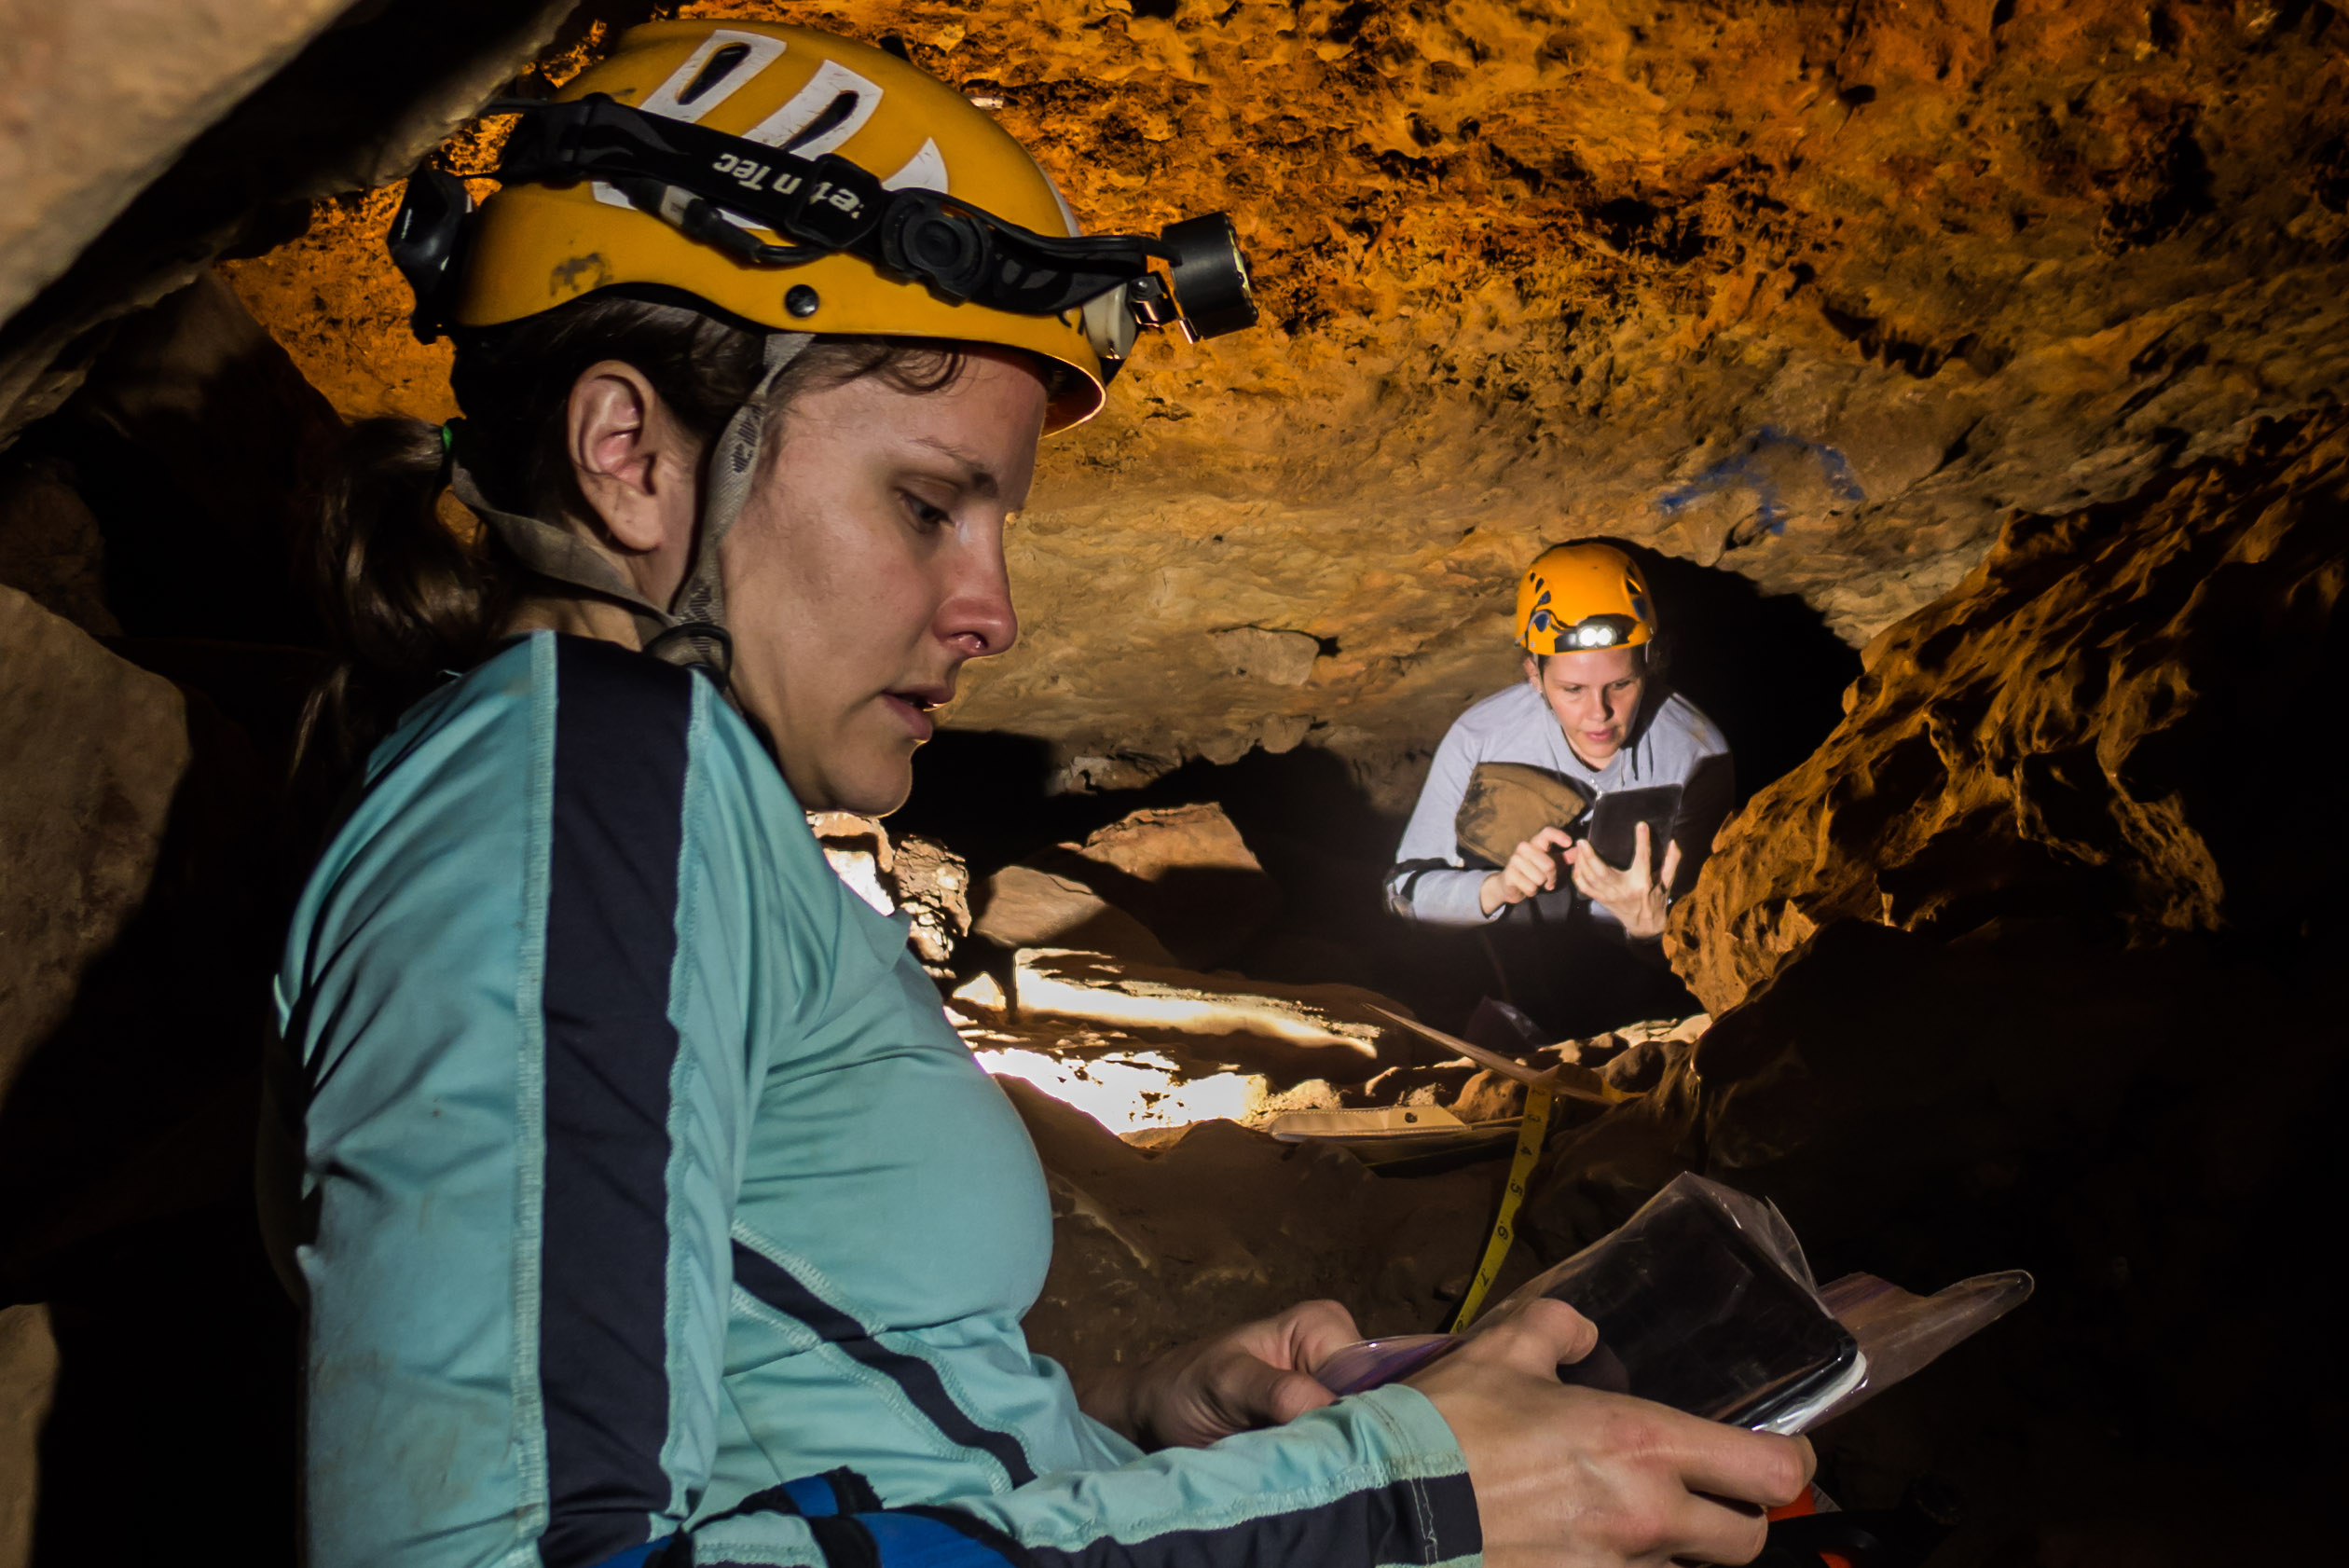
\includegraphics[width=\columnwidth]{cavewifi}

\subsection{Range experiment Software}
An Android application was developed to perform the range experiments in a cave and to test distances that could be achieved by Wifi Direct on a mobile device.
This initial application was developed based on a Wifi Direct example provided by the Android SDK.
The example was used to learn how to create the necessary Wifi Direct components, and understand how the significant asynchronous function calls operate together.
To perform the range experiments the example was modified to open a connection to a single device, load a data file from the device, and send the data file. 
The original application provided the ability for the client to launch the other devices photo gallery and select a photo to be copied.
This functionality was removed for the purposes of our experiment, and replaced with functionality that would allow us to transfer a true sample data file from a datalogger.

The Android application followed the architecture described in the section outlining the Android Wifi Direct APIs for creating peer to peer connections. 
The main application presents a fairly simple GUI interface allowing the user to kick off discovery. 
Upon completion of discovery a list of available peers is displayed on the GUI.
The user can then select from the list of devices which brings up a menu to connect to that device.
Once the Wifi Direct connection is established, the user may select a button to transfer the data file.
The GUI also provides the user a mechanism to take a note to be logged to a file so that data may be captured about the test being performed at the time.
The application timestamps the start and end of the data transfer and logs this information to a log file, in addition to any input the user provides from the GUI about the test.

\subsection{Data Ferry Software}
The data ferry software has currently been started, but is still under development.

\section{Results}

\subsection{Wifi Direct Range in Open Field}

We found a relatively open field in north Austin to carry out some range experiments with our Nexus 7 devices.
An open field, with no line of site obstructions and no other wifi devices around, should be the most ideal setting for Wifi direct ranges.
We started our tests at 100' apart and increases the distance by 50' to 100' at at time.
We found that our devices were easily able to connect and transfer a sample data file at distances up to 300' (91meters). 
We were able to connect and send the sample file at 350', 400', 500', and 600' (183m) with moderate success. 
At times, the connection would take longer than usual.
Also, the initial file transfer took multiple attempts.
Once the initial file was received, then subsequent transfers went much better.
However, at 650' (198m) the devices had a lot of trouble connecting, so we stopped measurements then.
This is very close to the claimed range of 200' meters.

\subsection{Wifi Direct Range in a Cave}
We gained access to Whirlpool Cave in south Austin with the permission of the managing entity, TCMA (http://www.tcmacaves.org/) and experimented with the range and connectivity of our Nexus 7 devices on March 16, 2014.


\subsection{Data Ferry Experiment Results}
This experiment has not yet been performed, and is planned to be completed before the final report.

\section{Conclusions and Future Work}
Currently the research is still underway, so this section will be completed in the final report.

\section{Acknowledgements}
TODO:
David Ochel - photography. 
TCMA and Matt Turner - access to Whirlpool Cave. 
Zara Environmental - sample data file.

% \begin{figure}[!b]
%   \begin{center}
%     \includegraphics[width=3.5in]{figure.pdf}
%   \end{center}
% 
%   \caption{\small Figure caption. To get a figure to span two columns, use the environment figure* rather than figure.}
%   \label{fig-label}
% \end{figure}

\bibliographystyle{abbrv}
\bibliography{refs}
\end{document}
